\pdfoutput=1
 \documentclass[aps, prapplied,twocolumn,showpacs,superscriptaddress,preprintnumbers, longbibliography,nofootinbib,floatfix]{revtex4-2}
\usepackage[normalem]{ulem}
\usepackage{amsmath}
\usepackage{amssymb}
\usepackage{physics}  % http://mirrors.ibiblio.org/CTAN/macros/latex/contrib/physics/physics.pdf
\usepackage{epsfig}

\usepackage{url} 

\usepackage{graphicx}
\usepackage{hyperref}
\usepackage{cleveref}
\crefname{figure}{Fig.}{Figs.}
\Crefname{figure}{Fig.}{Figs.}
\crefname{equation}{Eq.}{Eqs.}
\Crefname{equation}{Eq.}{Eqs.}
\crefname{section}{Sec.}{Secs.}
\Crefname{section}{Sec.}{Secs.}
%\usepackage{dcolumn}   % needed for some tables
\usepackage{tabu}
\usepackage{boldline}
\usepackage{xspace}
% \usepackage{titlingc
\usepackage{slashed}
\usepackage{multirow}
\usepackage{booktabs}
\usepackage{diagbox}
\usepackage{tabularx}
\usepackage{comment}
\usepackage{floatrow}
\newfloatcommand{capbtabbox}{table}[][\FBwidth]
\usepackage{color}
\usepackage[normal]{subfigure}
%\usepackage[margin=0.9in,a4paper]{geometry}
%\usepackage[table]{xcolor}
\usepackage{enumitem}
% \usepackage[utf8x]{inputenc}
\usepackage[utf8]{inputenc}
\usepackage[english]{babel}
%  \usepackage[compress,numbers,sort]{natbib}
%  \usepackage{authblk}3
\usepackage{colortbl}
\usepackage{upgreek}
\usepackage{lineno}
\linenumbers\relax  % line numbering 
\usepackage[separate-uncertainty=true]{siunitx}
\usepackage[dvipsnames]{xcolor}
\AtBeginDocument{\RenewCommandCopy\qty\SI}


\newcommand{\jt}[1]{\textcolor{blue}{[JT: #1]}}
\newcommand{\mb}[1]{\textcolor{ForestGreen}{[botti: #1]}}
\newcommand{\ab}[1]{\textcolor{teal}{[AB: #1]}}

\newcommand{\ansh}[1]{\textcolor{Fuchsia}{[ansh: #1]}}
\newcommand{\preliminary}[1]{\textcolor{red}{[#1]}}

\newcommand\sjt{\bgroup\markoverwith{\textcolor{blue}{\rule[0.5ex]{2pt}{0.4pt}}}\ULon}

\newcommand{\chd}{\marginpar{CHD}}

\captionsetup{justification=justified}
%\captionsetup{justification=justified}
\newcommand{\gf}{\textsc{Geant4}\xspace}
\DeclareCaptionJustification{justified}{\justified}

\renewcommand{\arraystretch}{1.15}
% Units Set-Up
\newcommand{\myqty}[3]{(\num{#1}~$\pm$~\num{#2})~\unit{#3}}  % \myqty{10}{1}{\metre} : (10 ± 1) m
\newcommand{\myrange}[3]{[\num{#1},~\num{#2}]~\unit{#3}}  % \myrange{4}{7}{\metre} : [4, 7] m
\newcommand{\avg}[1]{\left\langle #1 \right\rangle}

\sisetup{per-mode=symbol, inter-unit-product=\ensuremath{{}\cdot{}}}
\DeclareSIUnit{\electron}{e\textsuperscript{-}}
\DeclareSIUnit{\bar}{bar}
\DeclareSIUnit{\pix}{\textup{pixel}}
\DeclareSIUnit{\day}{\textup{day}}
\DeclareSIUnit{\epd}{\electron\per\pix\per\day}
\DeclareSIUnit{\ADU}{\text{A.D.U.}}


\usepackage{lipsum} 

\begin{document}


\preprint{}

\title{Long-Lived Charge Trap Characterization for Rare-Event Searches with Skipper-CCDs}

% ------------------------------------------------------
% ------------------------------------------------------

\author{Agustin Brusco}
% \email{agustin.brusco@gmail.com}
\affiliation{\normalsize\it 
Universidad de Buenos Aires, Facultad de Ciencias Exactas y Naturales, Departamento de Física, Buenos Aires, Argentina}

\author{Bruno Sivilotti}
% \email{brunosivilotti@hotmail.com}
\affiliation{\normalsize\it 
Universidad de Buenos Aires, Facultad de Ciencias Exactas y Naturales, Departamento de Física, Buenos Aires, Argentina}

\author{Ana M. Botti}
\affiliation{\normalsize\it 
Fermi National Accelerator Laboratory, PO Box 500, Batavia IL, 60510, USA}
\affiliation{\normalsize\it Kavli Institute for Cosmological Physics, University of Chicago, Chicago, IL 60637, USA}

\author{Brenda Cervantes}
\affiliation{\normalsize\it 
Fermi National Accelerator Laboratory, PO Box 500, Batavia IL, 60510, USA}

\author{Ansh Desai}
\affiliation{\normalsize\it 
Department of Physics and Institute for Fundamental Science, University of Oregon, Eugene, Oregon 97403, USA}

\author{Rouven Essig}
\affiliation{\normalsize\it 
C.N.~Yang Institute for Theoretical Physics, Stony Brook University, Stony Brook, NY 11794, USA}

 \author{Juan Estrada}
\affiliation{\normalsize\it 
Fermi National Accelerator Laboratory, PO Box 500, Batavia IL, 60510, USA}

\author{Erez Etzion}
\affiliation{\normalsize\it 
 School of Physics and Astronomy, Tel-Aviv University, Tel-Aviv 69978, Israel}
 
\author{Guillermo Fernandez Moroni}
\affiliation{\normalsize\it 
Fermi National Accelerator Laboratory, PO Box 500, Batavia IL, 60510, USA}

\author{Stephen E. Holland}
\affiliation{\normalsize\it Lawrence Berkeley National Laboratory, One Cyclotron Road, Berkeley, California 94720, USA}

\author{Ian Lawson}
\affiliation{\normalsize\it SNOLAB, Lively, ON P3Y 1N2, Canada}

\author{Steffon Luoma}
\affiliation{\normalsize\it SNOLAB, Lively, ON P3Y 1N2, Canada}

\author{Santiago E. Perez}
\affiliation{\normalsize\it 
Fermi National Accelerator Laboratory, PO Box 500, Batavia IL, 60510, USA}
\affiliation{\normalsize\it 
Universidad de Buenos Aires, Facultad de Ciencias Exactas y Naturales, Departamento de Física, Buenos Aires, Argentina}
\affiliation{\normalsize\it 
CONICET - Universidad de Buenos Aires, Instituto de Física de Buenos Aires (IFIBA). Buenos Aires, Argentina}

\author{Dario Rodrigues}
\affiliation{\normalsize\it 
Universidad de Buenos Aires, Facultad de Ciencias Exactas y Naturales, Departamento de Física, Buenos Aires, Argentina}
\affiliation{\normalsize\it 
CONICET - Universidad de Buenos Aires, Instituto de Física de Buenos Aires (IFIBA). Buenos Aires, Argentina}

\author{Javier Tiffenberg}
\affiliation{\normalsize\it 
Fermi National Accelerator Laboratory, PO Box 500, Batavia IL, 60510, USA}

\author{Sho Uemura}
\affiliation{\normalsize\it 
Fermi National Accelerator Laboratory, PO Box 500, Batavia IL, 60510, USA}

\author{Yikai Wu}
\affiliation{\normalsize\it 
C.N.~Yang Institute for Theoretical Physics, Stony Brook University, Stony Brook, NY 11794, USA}
\affiliation{\normalsize\it 
Department of Physics and Astronomy, Stony Brook University, Stony Brook, NY 11794, USA} 
% ------------------------------------------------------
% ------------------------------------------------------

\begin{abstract}
\noindent Skipper Charge-Coupled Devices (Skipper-CCDs) are detectors with sub-eV resolution, allowing them to play a critical role in rare event searches. 
A major challenge in experiments using these detectors is understanding and mitigating low-energy backgrounds which impact the single electron rate (SER). 
One potential component of the SER could arise from single-electron charge traps caused by lattice defects. 
In this work we present and use a new technique for generating uniform charge across the CCD to study single electron traps in a SENSEI sensor placed underground in the MINOS tunnel at Fermilab. 
The underground shielding allows us to make use of the pocket pumping technique to probe traps at high temperatures for long periods of time, allowing us to measure traps that would have emission times $>10^3$ seconds at normal operating temperatures. 
This is a regime not accessible in previous surface measurements of comparable sensors.
We fully characterize a significant fraction of the identified traps and use this information to extrapolate their contribution to the single-electron background in SENSEI.
\preliminary{We find that the studied population of traps does not significantly impact the single electron rate measured by SENSEI.}
% \noindent Skipper Charge-Coupled Devices (Skipper-CCDs) are ultra-low-threshold detectors capable of detecting energy deposits in silicon at the eV scale. Increasingly used in rare-event searches, one of the major challenges in these experiments is mitigating low-energy backgrounds. In this work, we present results on trap characterization in a silicon Skipper-CCD produced in the same fabrication run as the SENSEI experiment at SNOLAB. Lattice defects contribute to backgrounds in rare-event searches through single-electron charge trapping. To investigate this, we employ the charge-pumping technique at different temperatures to identify dipoles produced by traps in the CCD channel. We fully characterize a fraction of these traps and use this information to extrapolate their contribution to the single-electron background in SENSEI. We find that this subpopulation of traps does not contribute significantly but more work is needed to assess the impact of the traps that can not be characterized. 
\end{abstract}

\maketitle

\section{Traps and single-electron backgrounds}\label{sec:intro}
Skipper-Charge-Coupled-Devices (Skipper-CCDs) are pixelated silicon detectors that are widely used in rare-event searches~\cite{Smith2010, Holland:2003, Janesick1990,Wen1974}. 
They are enhanced versions of CCDs that can perform repeated non-destructive measurements of output charge and consequently achieve sub-electron resolution~\cite{Tiffenberg:2017aac}, enabling sensitivity to particles that produce one or a few electrons when they interact with the bulk silicon. 

The SENSEI and DAMIC experiments have achieved world leading results in the search for light dark matter, and significant efforts are underway to scale up these detectors and mitigate backgrounds~\cite{Abramoff:2019dfb, Sensei2020, SENSEI:2023zdf,DAMIC-M:2023gxo,aguilar2022oscura,DAMIC-M:2025luv}. 
These backgrounds may arise from environmental effects~\cite{Du_2022,Du:2023soy,Sensei2020} or intrinsic processes within the sensor~\cite{senseiSEE,ampLight}, and characterizing them will be key to maximizing sensitivity.

It is well known that defects can occur in the silicon from contaminants or vacancies that trap electrons (or holes) and release them after some time~\cite{claeys_metal_2018,pichler_intrinsic_2004,chroneos_oxygen_2015,wang_phosphorousvacancyoxygen_2013,collins_properties_1957,pintiliea_radiation_2009}. Due to these defects, charge from high energy backgrounds may become trapped and then released with a characteristic emission time $\tau_e$. If traps have sufficiently long $\tau_e$, they could produce uncorrelated single-electron events and therefore contribute to single-electron backgrounds. Results from the OSCURA collaboration~\cite{oscurasensors, trapsOscura} have indicated that elevated levels contaminants or defects were present in the silicon lattice of their Skipper-CCDs, motivating dedicated studies to understand the effects of possible defects in SENSEI CCDs on the SER.


Recently, measurements were performed at LAMBDA Laboratory at the University of Buenos Aires surface on a CCD fabricated from the same wafer as science-grade SENSEI CCDs~\cite{Brusco:2025kus}. These measurements suggested that current analysis strategies may mitigate the effect of charge traps. However, these measurements were taken at surface, thus were only sensitive to a certain range of trap lifetimes. This is because measurement times are limited due to the high rate of environmental and cosmic backgrounds at the surface. Generally, the emission time of charge traps decreases as a function of temperature, and thus to probe very long-lived traps (traps that emit electrons several days or even months after the initial trapping) at the usual operating temperature of $\sim135~K$ it is important to take longer measurements at higher operating temperatures, which must be done with dedicated measurements in a shielded underground setup. In this work we describe such a measurement, which we perform with SENSEI CCDs $\sim100~$m underground in the MINOS cavern at Fermi National Accelerator Laboratory (FNAL).

% The emission time of charge traps depends on its intrinsic energy (related to the source of the defect), its cross-section, and the temperature of the sensor. Emission time decreases exponentially as temperature increases. 


The Skipper-CCDs used in this study are made of high-resistivity silicon with an active area of 6144 $\times$ 1024 pixels each of size 15 $\times$ 15 $\mu$~m housed in a vacuum chamber equipped with a vacuum pump and a cryocooler. The CCD has four readout amplifiers that each read out in parallel a ``quadrant'' of 512 rows by 3072 columns. The CCD was operated and read out with a Low-Threshold-Acquisition board (LTA)~\cite{LTA}. In \cref{sec:measurement} we describe a new technique used to uniformly illuminate the CCD and the subsequent measurements taken to identify charge traps. We describe in \cref{sec:identification} how traps were identified and in \cref{sec:analysis} the trap energy and temperature dependence. We also perform data-driven simulation studies to study the accessible range of traps based on these measurements. We conclude in \cref{sec:discussion} with the impact of the trap density on single-electron backgrounds in SENSEI and compare with previous results.


\section{Charge Generation and Pocket-Pumping Measurements}\label{sec:measurement}
Unlike in the previous work, we did not use an LED to uniformly illuminate the CCD. Instead we took advantage of a feature inherent to CCDs known as spurious charge. Spurious charge is generated when the voltages of pixels in the active area are changed when shifting charge to neighboring pixels~\cite{janesick2001scientific}  The charge scales linearly with the number of shifts performed, and exponentially with the voltage clock swing, as expected from~\cite{janesick2001scientific}. Therefore by performing symmetric back-and-forth shifts with high voltage swing (charge-generating shifts), charge can be generated uniformly across the CCD in a controlled, reproducible manner. In this work we used a voltage swing of 10~V and 100,000 shifts to generate approximately $2000~e^-$ of charge per pixel. 

The pocket-pumping technique, described in detail in~\cite{trapsOscura} involves uniformly illuminating the CCD and then repeatedly moving the charge back and forth between the three pixel phases. If a trap exists in the edge phases, charges may be captured and released at a later time, spilling into the neighbor and creating a ``dipole'' signal relative to the uniform background. The number of charge carriers trapped and released, or in other words the intensity of the dipole ($I_{t_{ph}}$) is defined as half the difference in charge between the two pixels. The intensity depends on the number of pump cycles $N_{\text{pumps}}$ and the duration of each clock state $t_{ph}$.


The measurement procedure was as follows: for a given temperature, charge-generating shifts were performed as described above to uniformly illuminate the CCD with charge. Then the pocket-pumping protocol was performed with with $N_{\text{pumps}}=3000$ to obtain well-defined non-saturated dipoles for various $t_{ph}$. At a given temperature $t_{ph}$ was varied from approximately $5\times 10^{-5}$s to 1.03~s.  Only one skipper sample was taken to speed up readout time. Temperature was varied from \myrange{125}{210}{\kelvin} with 18-25 images at each temperature. We specifically took longer $t_{ph}$ measurements at higher temperatures to maximize sensitivity to longer trap emission times.

\section{Trap Characterization}
\label{sec:identification}
The dipole intensity depends on $N_{\text{pumps}}$, $t_{ph}$, the probability of capturing a charge carrier $P_c$ and the probability of emitting a charge carrier $P_e$~\cite{PhysRev.87.835,trapsOscura,HallPc}. $P_c$ acts a s a scaling factor that varies with temperature, and $P_e$ can be expressed as a function of the emission characteristic time $\tau_e(T)$. This gives:

\begin{align}\label{eq:I_fit}
    \mathrm{I(t_{ph}) =N_{pumps}D_t P_c \left(e^{-\frac{t_{ph}}{\tau_e}}-e^{-8\frac{t_{ph}}{\tau_e}}\right)}
\end{align}


Trap identification is performed using the same algorithm described in~\cite{Brusco:2025kus}. Once a trap is identified it was logged in each image taken at the same temperature, obtaining its intensity for each $t_{\text{ph}}$. For images taken at a given temperature ($T$) the intensity $I(t_{\text{ph}})$ of an identified trap for various delay times $t_{\text{ph}}$  can be plotted to predict the trap's emission time constant $\tau_e(T)$. If a trap only appears at one $t_{\text{ph}}$ value it is ignored. 

Fits are then performed according to \cref{eq:I_fit} for the identified traps. Following this criteria 60,029 dipoles are identified associated with 5171 traps. We analyze as before the spatial distribution of these identified traps using toy Monte-Carlo simulations. $10^4$ simulations were performed under the assumption of spatial uniformity. \cref{fig:trap_distribution} shows the histogram of the distances between all identified traps per quadrant, along with the simulation result and its corresponding 90\% confidence band assuming the traps are distributed uniformly. Some deviation from uniformity is expected due to the spatially localized nature of the cause of traps (defects in the CCD,  high energy events, etc), but in general we see good agreement with this simulation. 

\begin{figure}[!htb]
    \centering
    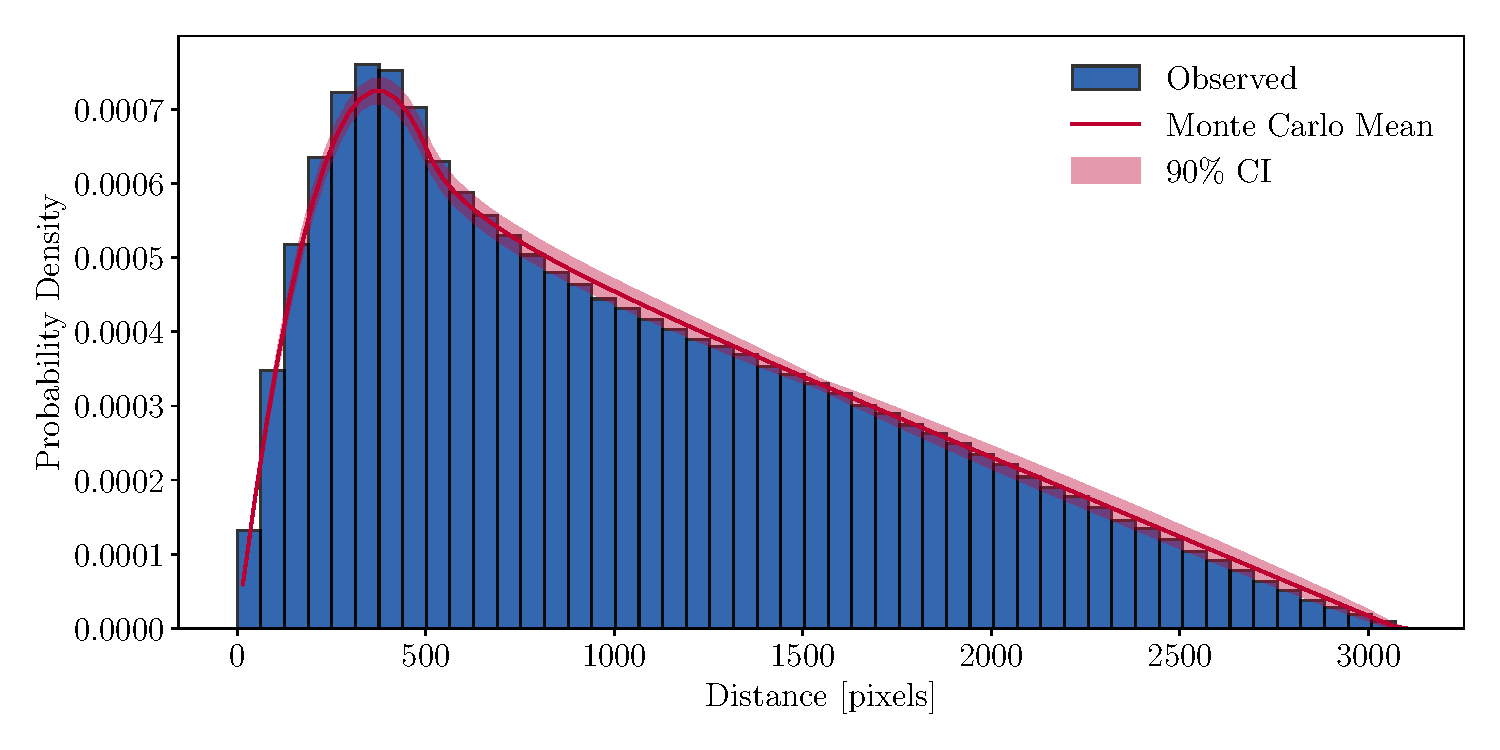
\includegraphics[width=\linewidth]{../figures/trap_distribution.pdf}
    \caption{Probability density of the distance between all identified traps, combining all four quadrants. The red curve and shaded band show the mean and 90\% confidence interval from $10^4$ toy Monte-Carlo simulations assuming a spatially uniform trap distribution. We see good agreement between the simulation and the data.}
    \label{fig:trap_distribution}
\end{figure}


A trap is identified as ``good'' if it meets the following criteria. First, the trap maximum intensity must be greater than 3$\sigma$, where $\sigma$ is the square root of the variance of the charge in the surrounding $35 \times 35$ pixels (trap should be bright enough). Second the relative error on the fit $\tau$ must be less than 50\% and the maximum of the intensity should be greater than three times the error on the intensity (the error bars shouldn't be too big.). Third, the p-value associated with the$\chi^2$ goodness of fit test should be greater than 0.05. Following this selection, 3379 traps are identified as ``good''. 



\ansh{should we talk about some of the bad traps we saw?}


\section{Trap temperature dependence and energy}\label{sec:analysis}
For a given charge trap we model the emission time $\tau_e$ as a function of lattice temperature $T$, the thermal velocity of the charge carriers $v_{th}$, the effective density of states in the conduction band $N_c$, the trap energy $E_c$ and the trap cross-section $\sigma$~\cite{PhysRev.87.835,trapsOscura,HallPc,Brusco:2025kus}. This gives:

\begin{align}\label{eq:tau(T)}
    \mathrm{\tau_e = \frac{1}{\sigma v_{th}N_c}e^{\frac{E_t}{k_B T}}},
\end{align}
where the temperature dependent $v_{th}$ and $N_c$ are defined as

\begin{align}
    \mathrm{v_{th} = \sqrt{\frac{3k_B T}{m_{cond}}}~~~and~~~
    N_c = 2 \left[ 2\pi m_{dens} \frac{k_B T}{h^2}\right]^{3/2}}.
\end{align}
\noindent here, h is the Plank's constant, $\mathrm{m_{cond} \simeq 0.41\,m_e}$ and $\mathrm{m_{dens} \simeq 0.94\,m_e}$ are the holes effective mass for conductivity and density of states respectively between 100 and 200\,K~\cite{GreenCon}, and $\mathrm{m_e}$ is the electron mass at rest.


For the traps identified as ``good,'' we further track the intensity fits for the same trap across different temperatures. By fitting all of these curves with \cref{eq:I_fit}, we can obtain $\tau_e$ for each trap as a function of the temperature T. This allows us to fit these measurements with \cref{eq:tau(T)}. We then mark a trap as ``well-behaved'' if they are within our analysis range, namely if they have at least four good temperature fits. Traps that do not satisfy this criteria either have behavior that does not match our model, or (more often) have emission time peaks that are either much shorter or much longer than the tested range. This further narrows down our total number of analyzed traps to 2121 ``well-behaved'' traps. An example of a well-behaved trap is shown in \cref{fig:good_trap}. 



\begin{figure}[!htb]
    \centering
    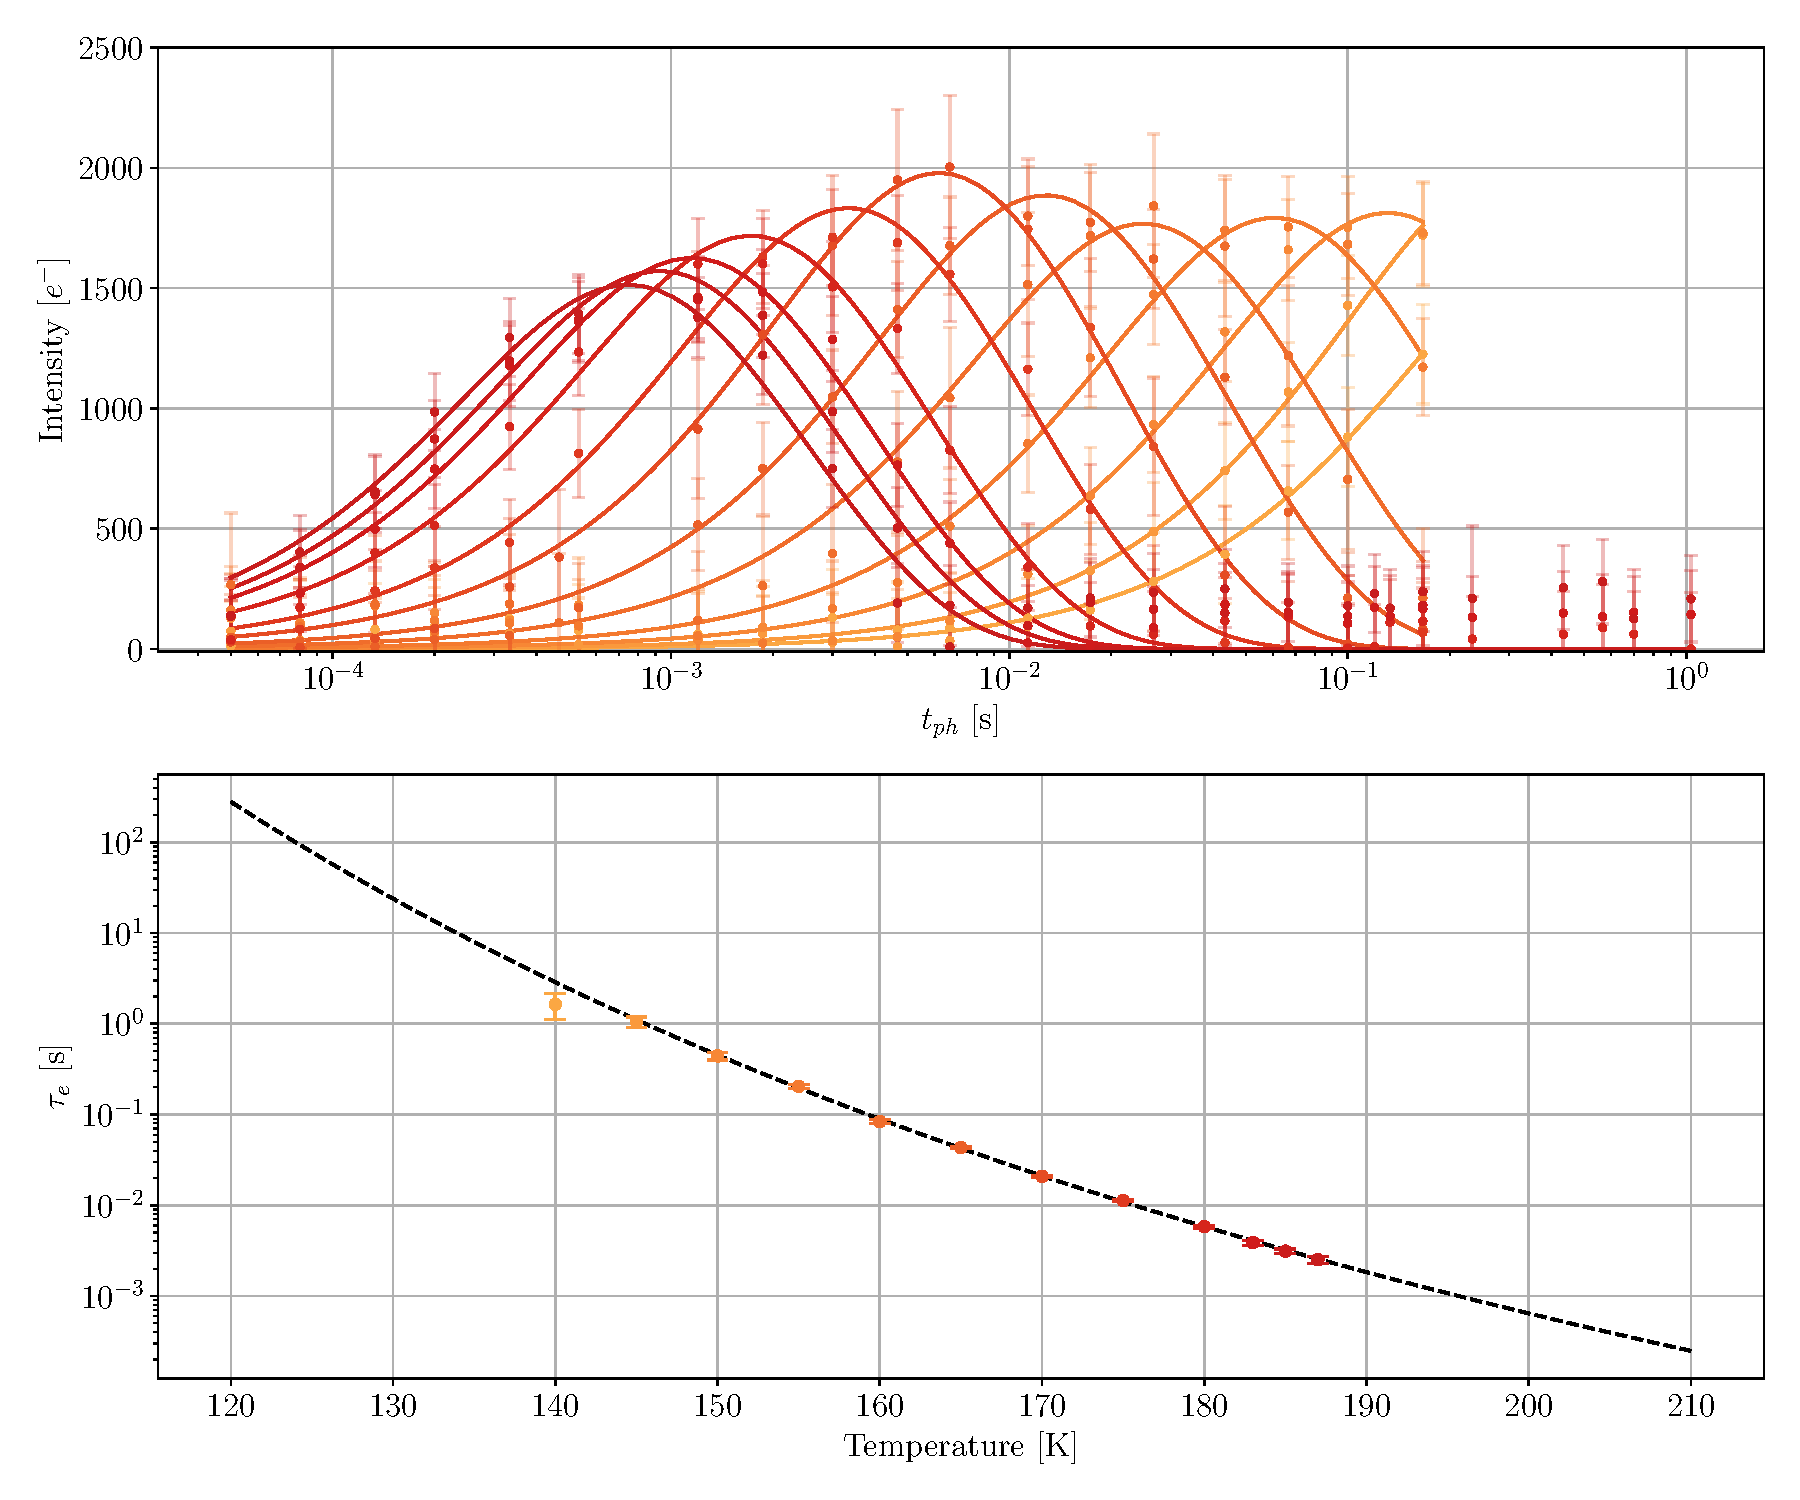
\includegraphics[width=\linewidth]{../figures/example_trap_3.pdf}
    \caption{An example of a well characterized charge trap in quadrant 1 of our CCD is shown. The \textbf{top} figure shows the intensity (in units of electron charge) vs $t_{ph}$ with error bars and the fit according to~\cref{eq:I_fit}. The \textbf{bottom} plot shows the temperature vs the fitted $\tau_e$ for the same trap with the fit line from~\cref{eq:tau(T)} The points are colored by temperature.}
    \label{fig:good_trap}
\end{figure}


We then fit according to \cref{eq:tau(T)} to find the energy and cross-section for these well-behaved traps.  We also observe two distinct populations. The first corresponds to the usual energies of standard defects $\sim0.2\,$eV (such as the $V_2$ vacancy~\cite{Wood_2014}), which we refer to as ``Group A'' ($\sim200$ traps)  and a second that peaks around $\sim0.5\,$eV, which we term ``Group B'' ($\sim50$ traps). This higher energy population was not previously accessible with the pocket-pumping technique.  As a reminder, the motivation of this work is to study the predicted backgrounds from charge traps at standard operating temperatures ($\sim$135~K), and of particular interest are the traps with very long emission times at such low temperatures. To study this region in particular, we took more measurements at high temperatures to extrapolate the emission time of these traps at low temperatures. \Cref{fig:all_traps} shows all of our energy and cross-section fits. The shaded gray region begins where we no longer have direct measurements of $\tau_e$ for any trap, all lines in this region are extrapolated from fitting with \cref{eq:tau(T)}. The white region denotes the measured trap emission times. The longer delay times and high temperature measurements done underground at MINOS allow us to probe significantly higher energies and cross-sections than were accessible previously~\cite{Brusco:2025kus}.

\begin{figure}[!htb]
    \centering
    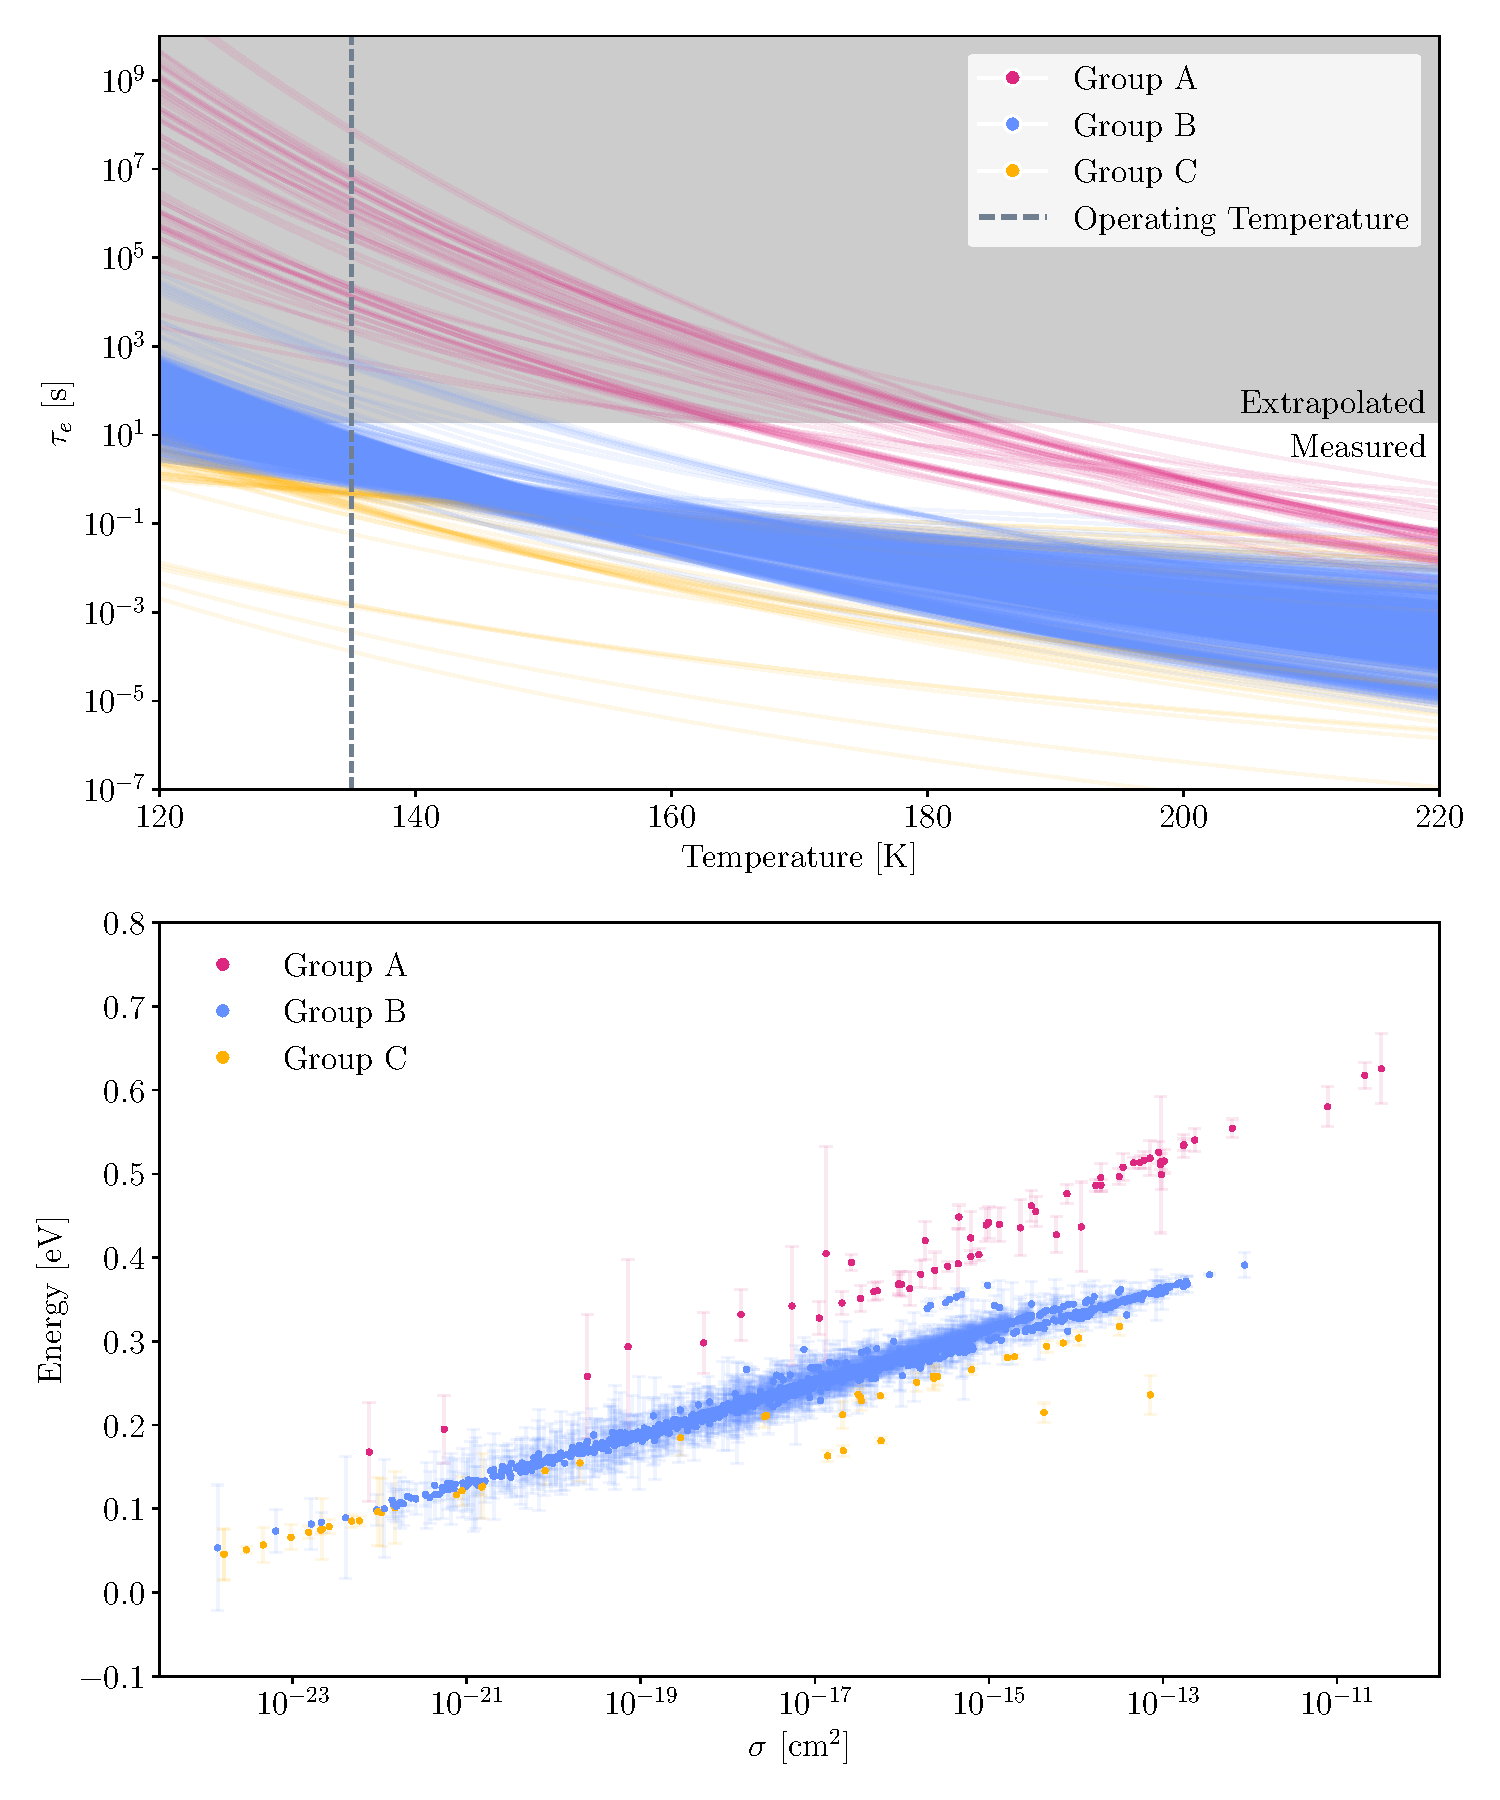
\includegraphics[width=\linewidth]{../figures/characterized_traps.pdf}
    \caption{All 2121 well-characterized traps, colored by observational group (A (pink): (measured above 170~K), B (blue): measured between 130-170~K,  and C (yellow): measured below 130~K). \textbf{Top}: Emission time $\tau_e$ as a function of temperature. Solid portions of each line indicate temperatures at which the trap was directly measured; the shaded gray region marks the extrapolated regime where no trap has a direct measurement at any temperature. The dashed vertical line marks the SENSEI@SNOLAB operating temperature of 135~K. \textbf{Bottom}: Fitted trap energy $E_t$ vs.\ capture cross-section $\sigma$ for the same traps.}
    \label{fig:all_traps}
\end{figure}


These fits were then used to predict the characteristic emission times for all well-behaved traps at 135~K, the typical operating temperature of SENSEI@SNOLAB~\cite{SENSEI:2023zdf}. This is shown in the top panel of \cref{fig:taue}. Here we see that we begin to measure some of the traps population with $\tau_e>1$~s, however a majority of the traps with longer delay times are extrapolated from observing these traps at high temperatures. We see that this distribution agrees with results from~\cite{Brusco:2025kus}. \ansh{should we say something about the shape of the distribution?}

Not all traps have direct $\tau_e$ measurements at every temperature. At a given temperature $T$, a trap's emission time is classified as \textit{measured} if for a given temperature there were enough measured values in the $t_{\text{ph}}$ range that $\tau_e$ was successfully fit at that temperature, and as \textit{extrapolated} if $\tau_e(T)$ is obtained solely from the fit to \cref{eq:tau(T)}. One can immediately see from the overlap between the measured and extrapolated trap emission times that there is some inefficiency of measuring a given trap. To understand why this inefficiency was taking place and to account for populations of traps that were not characterized at any temperature we perform a detailed data driven toy Monte-Carlo study. 

% We define the measurement efficiency $\varepsilon(\tau)$ as the fraction of trap emission times with a direct measurement in a given $\tau$ bin, pooled across all traps and all temperatures. This is shown in the bottom panel of \cref{fig:taue}. The efficiency reaches near unity for $\tau \sim 0.3$--1~s, reflecting the upper end of the $t_{\text{ph}}$ range, and falls to near zero for very short ($\tau \lesssim 10^{-5}$~s) and very long ($\tau \gtrsim 10^{3}$~s) emission times that lie outside our measurement window. This demonstrates that traps are only reliably measured within a particular range of $t_{\text{ph}}$.

% To test for traps that may have been missed due to measurement inefficiency, one can apply an efficiency correction to the $\tau_e(135~\text{K})$ histogram. For each trap, we do this by using evaluating the interpolated efficiency function $\varepsilon(\tau_e)$ for $\tau_e$ at the trap's mean measurement temperature. This allows us to scale the corresponding bin count by the inverse efficiency. We construct a conservative 90\% CL upper estimate of the trap population in each $\tau_e$(135~K) bin by applying a Poisson upper limit to the raw count and dividing by the measurement efficiency. The efficiency-corrected estimate and 90\% CL upper limit are shown in Fig.~\ref{fig:taue_upper_limit}, and are used as inputs to the simulation described in Section~\ref{sec:simulation}.

\begin{figure}[!htb]
    \centering
    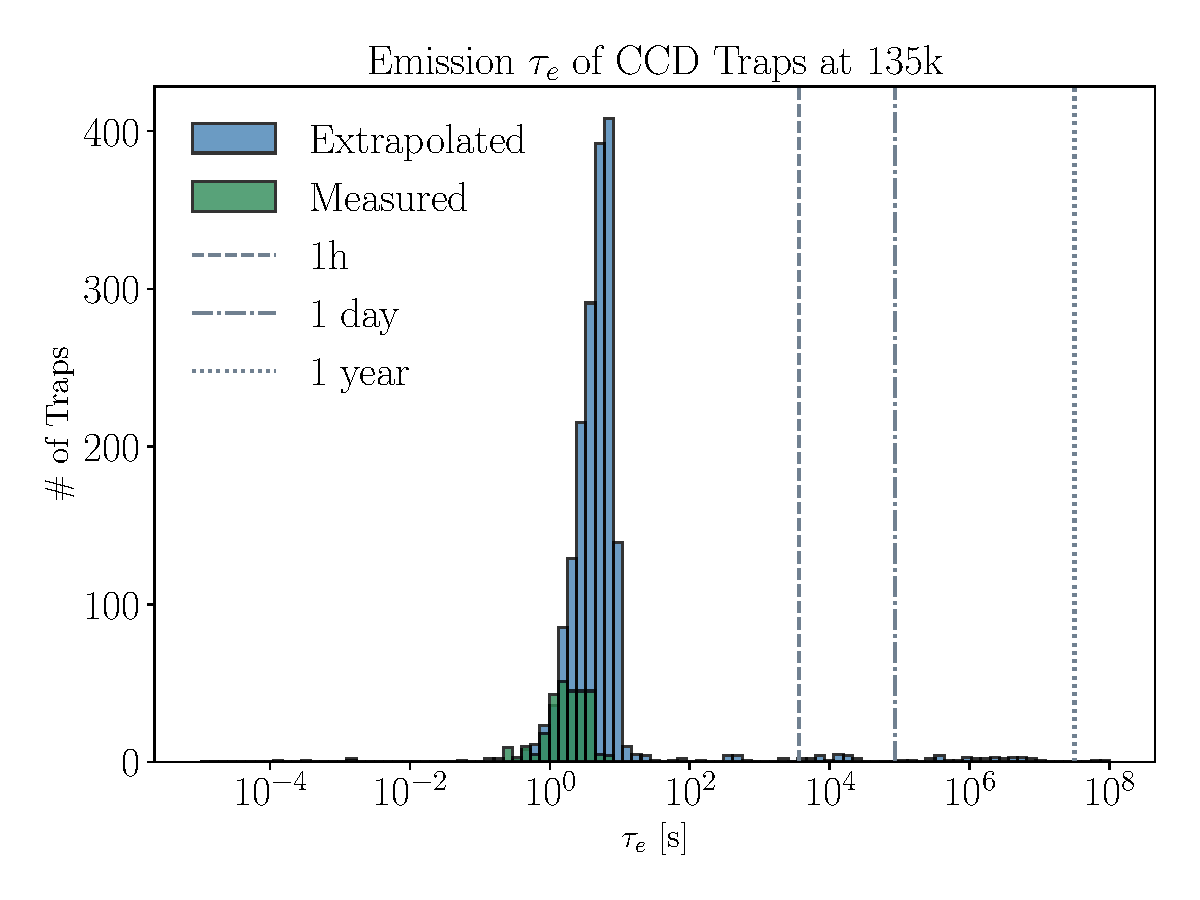
\includegraphics[width=\linewidth]{../figures/tau_at_135k_hist.pdf}
    % \subfigure{\includegraphics[width=\linewidth]{../figures/efficiency_tau_curve.pdf}\label{fig:efficiency}}
    \caption{\textbf{Top}: Histogram of the predicted emission time $\tau_e$ at 135~K for all 2121 well-characterized traps. Green bars indicate traps for which $\tau_e$ was directly measured; blue bars indicate traps extrapolated using \cref{eq:tau(T)}. Vertical lines mark 1~hour, 1~day, and 1~year. \textbf{Bottom}: Measurement efficiency $\varepsilon(\tau_e)$, defined as the fraction of trap emission times with a direct measurement in a given $\tau_e$ bin, pooled across all traps and all temperatures.} %Error bars reflect binomial uncertainty.
    \label{fig:taue}
\end{figure}

% \begin{figure}[!htb]
%     \centering
%     \includegraphics[width=\linewidth]{../figures/tau_at_135k_hist_upper_limit.pdf}
%     \caption{Estimated trap population at 135~K accounting for measurement efficiency. Blue bars show the raw known trap counts; red bars show the efficiency-corrected estimate obtained by dividing each bin by $\varepsilon(\tau)$ at the trap's mean measurement temperature; the hatched region shows the 90\% CL upper limit, derived from the Poisson upper limit on the raw counts divided by the same efficiency. Vertical lines mark 1~hour, 1~day, and 1~year.}
%     \label{fig:taue_upper_limit}
% \end{figure}


\section{Simulating Trap Emission}\label{sec:simulation}

To investigate the effect of these traps on our single-electron rate, an end-to-end simulation architecture capable of simulating SENSEI conditions was developed. A CCD is initialized with a given charge trap density (5171 traps / 6144 $\times$ 1024 pixels) and a given exposure-dependent and independent single-electron rate taken from SENSEI results~\cite{SENSEI:2024yyt}. Only one quadrant is simulated (3072 columns $times$ 512 rows). The traps themselves are randomly placed throughout the quadrant.  Each charge trap is assigned an emission time $\tau_e$ sampled from the distribution shown in \cref{fig:taue}.
For this work we take the exposure-dependent rate to be $4.36\times10^{-5}~e^-$/pix/day, and the exposure independent rate as $9.94\times10^{-5}~e^-$/pix/image. A ``fake'' image can then be taken for a given exposure. This randomly inserts single electron events calculated from a poissonian fluctuation around the predicted number of single electron events from the exposure-independent and exposure dependent rates. Then high energy events (referring to the actual event and a surrounding 60~pix radius) are sampled from a reference 20~h exposure SENSEI@MINOS image and then randomly placed in the simulated image. The number of high energy events is scaled linearly with exposure; for a 4~h image, a random 1/5 selection of the total high energy events are injected.  Then readout is simulated row by row with delay times corresponding to the actual time it takes to read out a full unbinned image. Trap interactions during each row-transfer dwell $dt$ follow two-state Shockley--Read--Hall kinetics: a trap captures a carrier from the charge packet above it at rate $\lambda_c = q\,\sigma v_{th}/V_p$, where $q$ is the packet occupancy, $\sigma$ the trap cross-section (sampled jointly with $\tau_e$ from the measured population), and $V_p$ the effective volume explored by a single carrier confined in the pixel well, and emits at rate $\lambda_e = 1/\tau_e$. Emitted carriers may be recaptured by the same trap before the packet is shifted away, so the trap state after each transfer is drawn from the exact two-state transition probabilities, $P_{\mathrm{release}} = \frac{\lambda_e}{\lambda_e+\lambda_c}\left(1-e^{-(\lambda_e+\lambda_c)\,dt}\right)$ and analogously for capture. We take $V_p = 3~\mu\mathrm{m}^3$ as the baseline, motivated by the collecting-phase area times the thermal vertical spread of a single carrier in the buried-channel well at 135~K; since inter-phase barriers far exceed $k_BT$ even at the small clock swings used in operation, $V_p$ is set by the well geometry rather than the clock amplitude. \ansh{numbers and figures in this section need to be regenerated with the updated trap interaction model (recapture) and a $V_p$ systematic variation} We assume unbinned SENSEI readout mode, where the total time to read out an image is $\sim$7~hours. Traps are allowed to remain trapped in one image and emit in future images. A single trial refers to an initialized CCD where a sequence of 5 images at exposure times of 0~h, 4~h, 6~h, 10~h, and 20~h is repeated 100 times, for a total of 500 images per trial. After images are taken, we apply a set of masks developed in previous analyses~\cite{Sensei2020,SENSEI:2023zdf,SENSEI:2024yyt}. We specifically apply the halo mask (60 pixel radius around pixel with $>100e^-$), vertical bleed mask (all pixels above pixel with $>100e^-$ are masked) and the hot column and hot pixel masks. As the latter two are data driven, to avoid truncation bias an A/B strategy is implemented, where half the simulation set is designated as set A, and the other half as set B. The set B statistics are used to decide the hot columns and pixels in A, and vice versa. 

After masking, the single electron densities are calculated for all exposures. They are then fit to obtain exposure-independent and exposure-dependent rates. To obtain sufficient statistics we take 500 such trials, resulting in 250,000 images. The simulation is run under two sets of observational conditions: MINOS conditions, corresponding to the environment of this study, and SNOLAB conditions, which assume a factor of 10 fewer high-energy events per exposure to reflect the greater overburden at SNOLAB~\cite{SENSEI:2023zdf}. For MINOS conditions using only the raw measured traps we find that with all masks applied the effect of traps on the exposure-independent rate is an increase of $\sim1.6\times10^{-7}$~$e^-$/pix/image, and the effect on the exposure-dependent rate is an increase of $1\times10^{-7}$~$e^-$/pix/day. The latter is consistent with zero within the simulation's statistical uncertainty, and the former is quite small. This can be seen in \cref{fig:minos_sim}.

\begin{figure}[!htb]
    \centering
    \includegraphics[width=\linewidth]{../figures/minos_conditions_sim_results.pdf}
    \caption{\textbf{Top:} Single-electron density as a function of exposure time under MINOS conditions, averaged over 500 trials. Red and blue points show the fitted exposure-independent and exposure-dependent rates with and without traps respectively; the dashed line shows the injected truth. The bottom panel shows the per-exposure difference between the with-trap and without-trap fits. The effect of traps on the exposure-independent rate is $\sim$$2\times10^{-7}$~$e^-$/pix/image, and the effect on the exposure-dependent rate is negligible.\textbf{Bottom:} The difference between the simulation with trap effects and the simulation without trap effects is shown. The effect is roughly proportional to exposure, with the 0 hour exposure slightly inflated due to the ordering of the measurement protocol.}
    \label{fig:minos_sim}
\end{figure}

The simulation is additionally run using the 90\% CL upper limit trap distribution as the trap input, to bound the impact of uncharacterized traps. The results of all four scenarios — MINOS and SNOLAB conditions, each with the baseline and upper-limit trap distributions — are summarized in \cref{fig:results_comparison}. Across all scenarios, the effect on both the exposure-independent and exposure-dependent rates remains small. Under the upper-limit trap assumption, the largest shifts are $\sim2.2\times10^{-7}$~$e^-$/pix/image in the exposure-independent rate and $\sim4.2\times10^{-7}$~$e^-$/pix/day in the exposure-dependent rate, both below 1\% of the rate measured in~\cite{SENSEI:2024yyt}. We see that for SNOLAB conditions the increase is negligible for the exposure independent case, and roughly consistent with the MINOS results in the exposure dependent case. 

\begin{figure}[!htb]
    \centering
    
\includegraphics[width=\linewidth]{../figures/results_comparison.pdf}
    \caption{Comparison of fitted single-electron rates across all four simulation scenarios. Filled (open) markers indicate MINOS (SNOLAB) conditions; red (blue) markers indicate simulations with (without) traps. Results are shown for both the baseline trap distribution (bottom two rows) and the 90\% CL upper limit (top two rows). The dashed vertical line marks the injected truth. \textbf{Top}: Exposure-independent rate. \textbf{Bottom}: Exposure-dependent rate.}
    \label{fig:results_comparison}
\end{figure}

As this was the same CCD as used to compare results in~\cite{SENSEI:2024yyt} we were able to directly test the impact of masking these traps on our measured $1e^-$ rate. We see that masking all 5171 detected traps had no significant impact on our $1e^-$ rate, supporting previous results suggesting that our masking procedures are effective at removing this background \ansh{though I guess it would only catch the ones that emit fast and therefore look like hot pixels}. Without masking the effective increase for MINOS conditions (MINOS conditions assuming the upper limit) is $\sim2\times10^{-5}~e^-$/pix/image (($\sim3\times10^{-5}~e^-$/pix/image)for the exposure independent rate and $4\times10^{-4}~e^-$/pix/day ($5\times10^{4}~e^-$/pix/day) for exposure dependent rate. This is a significant increase from the baseline, highlighting the effectiveness of masking in mitigating backgrounds from these effects. 


\ansh{benchmark of the increase in 1e rate without masking from this background is missing for upper limit version, so i left those as blank parentheses above}





\section{Summary and outlook}\label{sec:discussion}

In this work we characterized charge traps in a science-grade SENSEI Skipper-CCD operated underground in the MINOS cavern at Fermilab. We introduced a new technique for uniformly illuminating the CCD using spurious charge generated by symmetric clock swings, removing the need for an external light source. We then applied the pocket-pumping measirement technique over $125$--$210$~K and identified 5171 traps. We fully characterized a large fraction of these at very high temperatures and long swing, which was made possible by environmental shielding provided by the MINOS cavern. This allowed us to probe trap emission times of hundreds of days at the SENSEI@SNOLAB operating temperature of 135~K, a regime previously inaccessible.

The characterized traps cluster predominantly at $\tau_e \sim 10^{-1}$--$10^{2}$~s at 135~K, with a tail extending to multi-day lifetimes. To bound the contribution of traps that fall outside our measurement window at all temperatures, we introduced a measurement efficiency $\varepsilon(\tau)$ pooled across all traps and temperatures, and derived a 90\% CL upper limit on the trap population in each $\tau$ bin. This provides a quantitative bound on the contribution of the uncharacterized population that complements the direct characterization.

We tested both the directly-measured and the 90\% CL upper-limit trap distributions with an end-to-end CCD simulation under MINOS and SNOLAB conditions. With the standard SENSEI masking applied and under the upper limit assumption, the trap-induced shift in the single-electron rate is at most $\sim2\times10^{-7}$~$e^-$/pix/image in the exposure-independent component and $\sim4\times10^{-7}$~$e^-$/pix/day in the exposure-dependent component, in both cases below 1\% of the rate measured in the most recent SENSEI@SNOLAB analysis~\cite{SENSEI:2024yyt}. The shifts under SNOLAB conditions are $2$--$3\times$ smaller than under MINOS conditions, consistent with the picture that this background is sourced by charge from high-energy events being temporarily stored in traps and later released; deeper overburden suppresses the trap-mediated background alongside the primary one. This supports the conclusion of Ref.~\cite{Brusco:2025kus} that current masking strategies effectively mitigate this source of background.

These results demonstrate the value of characterizing charge traps for single-electron-sensitive experiments, and will be especially relevant for upcoming large-scale efforts such as DAMIC-M and Oscura. The spurious-charge illumination technique demonstrated here is well-suited to characterize traps in all sensors of such experiments simultaneously, without dedicated test stands. Since the trap population is expected to depend on fabrication, repeating these measurements on each new sensor batch will be important. We delegate an investigation of the traps that did not meet our fit criteria to future work, and note that understanding these populations may further refine our picture of defect-induced backgrounds in skipper-CCDs.

\begin{acknowledgments}
We are grateful for the support of the Heising-Simons Foundation under Grant No.~79921. This document was prepared by the SENSEI collaboration using the resources of the Fermi National Accelerator Laboratory (Fermilab), a U.S. Department of Energy, Office of Science, Office of High Energy Physics HEP User Facility. Fermilab is managed by Fermi Research Alliance, LLC (FRA), acting under Contract No.~DE-AC02-07CH11359.
The CCD development work was supported in part by the Director, Office of Science, of the DOE under No.~DE-AC02-05CH11231.
The U.S. Government retains and the publisher, by accepting the article for publication, acknowledges that the U.S. Government retains a non-exclusive, paid-up, irrevocable, world-wide license to publish or reproduce the published form of this manuscript, or allow others to do so, for U.S. Government purposes.
\end{acknowledgments}
%We acknowledge the invaluable support of the public and free university system, curcial in this research. This work was supported by Fermilab under DOE Contract No. DE-AC02-07CH11359. The CCD development work was supported in part by the Director, Office of Science, of the DOE under No. DE-AC02-05CH11231. We are grateful for the support of the Heising-Simons Foundation under Grant No. 79921. %This manuscript has been authored by Fermi Research Alliance, LLC under Con- tract No. DE-C02-07CH11359 with the U.S. Depart-ment of Energy, Office of Science, Office of High Energy Physics. The United States Government retains and the publisher, by accepting the article for publication, acknowledges that the United States Government retains a non-exclusive, paid-up, irrevocable, world-wide license to publish or reproduce the published form of thismanuscript, or allow others to do so, for United States Government purposes.


%\bibliography{apssamp}% Produces the bibliography via BibTeX.
%\bibliographystyle{apsrev4-1-b.bst}
%\bibliography{Compton.bib}

%\appendix

%\section{Appendixes}
%\bibliographystyle{apsrev4-1-b.bst}
\bibliography{references.bib}
%\bibliography{sensei.bib}

\end{document}
%
% ****** End of file apssamp.tex ******
